\documentclass[a4paper,12pt]{article}
\usepackage[utf8]{inputenc}
\usepackage[ngerman]{babel}
\usepackage{amsmath}
\usepackage{amssymb}
\usepackage{amsthm}
\usepackage{geometry}
\usepackage{graphicx}
\usepackage[hidelinks]{hyperref}
\usepackage{listings}
\usepackage{xcolor}
\usepackage{enumitem}
\usepackage[activate={true,nocompatibility},final,tracking=true,kerning=true,spacing=true,factor=1100,stretch=10,shrink=10]{microtype}
\usepackage{booktabs}
\usepackage{caption}
\usepackage{url}

\geometry{margin=2.5cm}
\sloppy

\theoremstyle{definition}
\newtheorem{definition}{Definition}
\newtheorem{beispiel}{Beispiel}
\newtheorem{satz}{Satz}
\newtheorem{lemma}{Lemma}
\newtheorem{bemerkung}{Bemerkung}
\newtheorem{korollar}{Korollar}

\setlist[itemize,1]{label=--}

% ---------- Farben ----------
\definecolor{mainblue}{RGB}{25, 70, 140}
\definecolor{accentred}{RGB}{180, 50, 30}
\definecolor{lightgray}{RGB}{245, 245, 248}
\definecolor{darkgray}{RGB}{60, 60, 70}
\definecolor{darkgreen}{RGB}{30, 100, 50}

\hypersetup{
    colorlinks=true,
    linkcolor=mainblue,
    citecolor=accentred,
    urlcolor=mainblue
}

\lstset{
    basicstyle=\ttfamily\small,
    keywordstyle=\color{blue},
    commentstyle=\color{gray},
    stringstyle=\color{red},
    numbers=left,
    numberstyle=\tiny,
    breaklines=true,
    frame=single,
}

\newcommand{\mydegree}{^\circ}

\title{Energiegewinnung durch geomagnetische Induktion:\\
Formale Analyse der s\"akularen Variation und\\
geomagnetischer St\"urme als Induktionsquellen}
\author{Stephan Epp}
\date{20. Juni 2026}

\begin{document}

\maketitle

\begin{abstract}
Das Erdmagnetfeld unterliegt permanenten zeitlichen Ver\"anderungen, die durch
die s\"akulare Variation, solaren Einfluss und geomagnetische St\"urme
hervorgerufen werden. Diese Arbeit untersucht formal die M\"oglichkeit,
elektrische Energie durch elektromagnetische Induktion aus diesen Magnetfeldver\"ander\-ungen zu gewinnen.
Es werden die relevanten physikalischen Gesetze hergeleitet, quantitative Absch\"atzungen
der induzierten Spannungen und Leistungen f\"ur verschiedene Szenarien durchgef\"uhrt
sowie die praktischen Grenzen und technischen Anforderungen rigoros nachgewiesen.
Die Analyse zeigt, dass s\"akulare Variation allein technisch nicht nutzbar ist,
geomagnetische St\"urme hingegen bei sehr gro{\ss}fl\"achigen Induktionssystemen
messbare und prinzipiell nutzbare elektrische Energiemengen erzeugen k\"onnen.
\end{abstract}

\tableofcontents
\newpage

% ═══════════════════════════════════════════════════════════════
\section{Einf\"uhrung}

Das Erdmagnetfeld ist eines der fundamentalsten Naturph\"anomene unseres Planeten.
Es sch\"utzt die Biosph\"are vor dem Sonnenwind, erm\"oglicht Navigation und
beeinflusst die Ionosph\"are. Weniger bekannt ist, dass das Erdmagnetfeld kein
statisches Feld ist, sondern st\"andigen Schwankungen unterliegt -- auf Zeitskalen
von Sekunden bis zu zehntausenden von Jahren.

Das Faraday'sche Induktionsgesetz besagt, dass jede zeitliche \"Anderung eines
Magnetflusses eine elektromotorische Kraft (EMK) induziert. Daraus ergibt sich
die nat\"urliche Frage: L\"asst sich die geomagnetische Variation als Energiequelle nutzen?

\subsection{Problemstellung}

Gegeben ist ein zeitlich ver\"anderliches Magnetfeld $\mathbf{B}(t)$ der Erde.
Eine planare Leiterschleife mit Fl\"ache $A$ und $N$ Windungen ist im Raum
orientiert. Gesucht sind:

\begin{itemize}
    \item Die induzierte elektromotorische Kraft $\varepsilon(t)$ als Funktion
          der Magnetfeldvariationsrate $\tfrac{\mathrm{d}B}{\mathrm{d}t}$
    \item Die maximal nutzbare Leistung $P_{\max}$ bei gegebener Lastimpedanz
    \item Die Mindestfl\"ache $A_{\min}$, ab der eine technisch relevante
          Spannung (hier: $\varepsilon \geq 1\,\mathrm{V}$) erreicht wird
    \item Ein quantitativer Vergleich verschiedener geomagnetischer Variationsquellen
\end{itemize}

\subsection{Motivation}

Die Gewinnung elektrischer Energie aus nat\"urlichen Magnetfeldvariationen
k\"onnte in abgelegenen Regionen ohne Netzanschluss oder f\"ur
Sensornetzwerke mit extrem geringem Energiebedarf von Interesse sein.
Insbesondere geomagnetische St\"urme, die mehrmals j\"ahrlich auftreten,
erzeugen Magnetfeldvariationen, die in historischen F\"allen gro{\ss}e
Auswirkungen auf elektrische Infrastruktur hatten -- ein Indiz, dass
erhebliche Energiemengen im Spiel sind.

Ferner bildet diese Untersuchung die theoretische Grundlage f\"ur das
Verst\"andnis geomagnetisch induzierter Str\"ome (GIC), die f\"ur
den Schutz von Stromnetzen und Pipelines relevant sind.

% ═══════════════════════════════════════════════════════════════
\section{Grundlagen}

\subsection{Physikalische Definitionen}

\begin{definition}[Magnetischer Fluss]
    Der magnetische Fluss $\Phi$ durch eine ebene Fl\"ache $A$ mit
    Normalenvektor $\hat{n}$ in einem homogenen Magnetfeld $\mathbf{B}$ ist:
    \[
        \Phi = \mathbf{B} \cdot A \cdot \hat{n} = B \cdot A \cdot \cos\varphi
    \]
    wobei $\varphi$ der Winkel zwischen $\mathbf{B}$ und $\hat{n}$ ist.
    Die SI-Einheit ist das Weber: $[\Phi] = \mathrm{Wb} = \mathrm{V\,s}$.
\end{definition}

\begin{definition}[Elektromagnetische Induktion (Faraday)]
    Die induzierte elektromotorische Kraft $\varepsilon$ in einer Leiterschleife
    ist gleich der negativen zeitlichen \"Anderungsrate des magnetischen Flusses:
    \[
        \varepsilon = -\frac{\mathrm{d}\Phi}{\mathrm{d}t}
    \]
    F\"ur $N$ Windungen gilt entsprechend:
    \[
        \varepsilon = -N \cdot \frac{\mathrm{d}\Phi}{\mathrm{d}t}
    \]
\end{definition}

\begin{definition}[S\"akulare Variation]
    Die s\"akulare Variation bezeichnet die langsame, kontinuierliche \"Anderung
    des geomagnetischen Feldes auf Zeitskalen von Jahren bis Jahrtausenden,
    hervorgerufen durch Str\"omungsprozesse im fl\"ussigen \"au{\ss}eren Erdkern.
    Typische Werte betragen $10$--$80\,\mathrm{nT/Jahr}$.
\end{definition}

\begin{definition}[Geomagnetischer Sturm]
    Ein geomagnetischer Sturm ist eine vor\"ubergehende st\"arke St\"orung
    des Erdmagnetfeldes, ausgel\"ost durch koronale Massenausw\"urfe (CME)
    der Sonne. Die Hauptphase ist durch einen starken Abfall des Ringstroms
    gekennzeichnet. Die Amplitude des $D_{st}$-Index erreicht
    bei moderaten Ereignissen $-50$ bis $-100\,\mathrm{nT}$,
    bei extremen Ereignissen (wie dem Carrington-Ereignis 1859) vermutlich
    mehr als $-1600\,\mathrm{nT}$.
\end{definition}

\begin{definition}[Geomagnetisch induzierter Strom (GIC)]
    Geomagnetisch induzierte Str\"ome entstehen, wenn \"Anderungen des
    Erdmagnetfeldes in ausgedehnten leitenden Strukturen (Pipelines,
    Strom\"ubertragungs\-leitungen) elektrische Str\"ome induzieren.
    Sie folgen direkt dem Faraday-Gesetz angewendet auf die nat\"urliche
    Leiterschleife, die die Infrastruktur mit dem Erdboden bildet.
\end{definition}

\subsection{Das Erdmagnetfeld}

Das Erdmagnetfeld ist ein Dipolfeld erster N\"aherung. Seine charakteristischen
Gr\"o{\ss}en an der Erdoberfl\"ache sind:

\begin{itemize}
    \item Gesamtintensit\"at: $B \approx 25\,000$--$65\,000\,\mathrm{nT}$
          (\"Aquator vs. Pole)
    \item Horizontalkomponente am \"Aquator: $H \approx 30\,000\,\mathrm{nT}$
    \item Inklination: $0^{\circ}$ am geomagnetischen \"Aquator, $\pm 90^{\circ}$
          an den geomagnetischen Polen
    \item Referenzwert f\"ur Rechnungen: $B_0 = 50\,000\,\mathrm{nT} = 50\,\mathrm{\mu T}$
\end{itemize}

\subsection{Quellen zeitlicher Magnetfeldvariationen}

Tabelle~\ref{tab:quellen} fasst die wichtigsten Quellen geomagnetischer
Variationen mit ihren charakteristischen Amplituden und Zeitskalen zusammen.

\begin{table}[h!]
\centering
\caption{Quellen geomagnetischer Variationen}
\label{tab:quellen}
\begin{tabular}{lrrl}
\toprule
\textbf{Quelle} & \textbf{Amplitude} & \textbf{Zeitskala} & \textbf{Anmerkung} \\
\midrule
S\"akulare Variation      & $10$--$80\,\mathrm{nT}$   & Jahre          & Kontinuierlich \\
Tagesschwankung (Sq)      & $10$--$100\,\mathrm{nT}$  & $\sim 24\,\mathrm{h}$  & Ionosph\"are \\
Mondtide (L-Variation)    & $2$--$5\,\mathrm{nT}$     & $\sim 25\,\mathrm{h}$  & Schwach \\
Geomagnet. Sturm (moderat)& $100$--$500\,\mathrm{nT}$ & Stunden        & Mehrmals/Jahr \\
Geomagnet. Sturm (extrem) & $>1000\,\mathrm{nT}$      & Minuten        & Selten \\
Erdbebenvorläufer (ULF)   & $1$--$10\,\mathrm{nT}$    & Sekunden       & Umstritten \\
Carrington-Ereignis (1859)& $\gg 1600\,\mathrm{nT}$  & Minuten        & Historisch max. \\
\bottomrule
\end{tabular}
\end{table}

% ═══════════════════════════════════════════════════════════════
\section{Formale Herleitung der Induktionsgleichungen}

\subsection{Grundlegende Herleitung}

Sei $\mathbf{B}(t) = B(t)\,\hat{z}$ ein zeitlich ver\"anderliches, r\"aumlich
homogenes Magnetfeld in $z$-Richtung. Eine horizontale, planare Spule mit
Fl\"ache $A$ und $N$ Windungen liegt in der $xy$-Ebene, sodass $\hat{n} = \hat{z}$
und $\cos\varphi = 1$.

\begin{satz}[Induzierte Spannung bei geomagnetischer Variation]
\label{satz:induktion}
    F\"ur eine planare Spule mit Fl\"ache $A$ und $N$ Windungen, die senkrecht
    zum Erdmagnetfeld orientiert ist, gilt f\"ur die induzierte EMK:
    \[
        \varepsilon(t) = -N \cdot A \cdot \frac{\mathrm{d}B}{\mathrm{d}t}
    \]
\end{satz}

\begin{proof}
    Der magnetische Fluss durch eine Windung betr\"agt nach Definition~1:
    \[
        \Phi(t) = B(t) \cdot A \cdot 1 = B(t) \cdot A
    \]
    F\"ur $N$ Windungen gilt der Gesamtfluss $\Psi = N \cdot \Phi(t)$.
    Das Faraday'sche Induktionsgesetz (Definition~2) liefert:
    \[
        \varepsilon(t) = -\frac{\mathrm{d}\Psi}{\mathrm{d}t}
        = -\frac{\mathrm{d}(N \cdot B(t) \cdot A)}{\mathrm{d}t}
        = -N \cdot A \cdot \frac{\mathrm{d}B}{\mathrm{d}t}
    \]
    da $N$ und $A$ zeitunabh\"angig sind.
\end{proof}

\subsection{Maximale Leistungs\"ubertragung}

\begin{satz}[Maximum-Power-Transfer-Theorem f\"ur den geomagnetischen Induktor]
\label{satz:leistung}
    Eine Spule mit Innenwiderstand $R_i$ und induzierter EMK $\varepsilon$
    \"ubertr\"agt maximale Leistung an einen Lastwiderstand $R_L$, wenn
    $R_L = R_i$. Die maximale Nutzleistung betr\"agt:
    \[
        P_{\max} = \frac{\varepsilon^2}{4 R_i}
    \]
\end{satz}

\begin{proof}
    Die Leistung an der Last ist:
    \[
        P(R_L) = \left(\frac{\varepsilon}{R_i + R_L}\right)^2 \cdot R_L
        = \varepsilon^2 \cdot \frac{R_L}{(R_i + R_L)^2}
    \]
    Ableitung nach $R_L$ und Nullsetzung:
    \[
        \frac{\mathrm{d}P}{\mathrm{d}R_L}
        = \varepsilon^2 \cdot \frac{(R_i + R_L)^2 - 2R_L(R_i+R_L)}{(R_i+R_L)^4}
        = \varepsilon^2 \cdot \frac{R_i - R_L}{(R_i+R_L)^3} \overset{!}{=} 0
    \]
    Daraus folgt $R_L = R_i$. Einsetzen ergibt:
    \[
        P_{\max} = \varepsilon^2 \cdot \frac{R_i}{(2R_i)^2} = \frac{\varepsilon^2}{4R_i}
    \]
\end{proof}

\subsection{Widerstand einer Flachspule}

F\"ur eine rechteckige Spule der Seitenl\"ange $\ell = \sqrt{A}$ mit $N$ Windungen
aus Kupferdraht des Querschnitts $q$ gilt:

\begin{lemma}[Innenwiderstand der Flachspule]
\label{lem:widerstand}
    Der Innenwiderstand einer planaren quadratischen Spule mit Fl\"ache $A$,
    $N$ Windungen und Drahtquerschnitt $q$ aus Kupfer
    ($\rho_{Cu} = 1{,}68 \times 10^{-8}\,\Omega\,\mathrm{m}$) betr\"agt:
    \[
        R_i = \frac{4 \rho_{Cu} \cdot N \cdot \sqrt{A}}{q}
    \]
\end{lemma}

\begin{proof}
    Die Gesamtl\"ange des Drahtes betr\"agt f\"ur $N$ quadratische Windungen
    mit ungef\"ahr gleicher Seitenl\"ange $\ell = \sqrt{A}$:
    \[
        L_{\text{Draht}} \approx 4N\sqrt{A}
    \]
    Der elektrische Widerstand folgt aus $R = \rho \cdot L / q$:
    \[
        R_i = \frac{\rho_{Cu} \cdot 4N\sqrt{A}}{q}
    \]
\end{proof}

\begin{korollar}[Optimaler Drahtquerschnitt]
    Aus Satz~\ref{satz:leistung} und Lemma~\ref{lem:widerstand} folgt:
    Die Nutzleistung ist unabh\"angig von der Windungszahl $N$, wenn
    der Gesamtmaterialeinsatz (Gesamtvolumen des Kupfers) konstant gehalten wird,
    da $\varepsilon \propto N$ und $R_i \propto N$ sich herausk\"urzen.
\end{korollar}

\begin{proof}
    Sei $V_{Cu} = N \cdot 4\sqrt{A} \cdot q = \text{const.}$, also $q = V_{Cu}/(4N\sqrt{A})$.
    Dann gilt:
    \[
        R_i = \frac{4\rho_{Cu} N \sqrt{A}}{q}
        = \frac{4\rho_{Cu} N \sqrt{A} \cdot 4N\sqrt{A}}{V_{Cu}}
        = \frac{16\rho_{Cu} N^2 A}{V_{Cu}}
    \]
    und $\varepsilon = N A \tfrac{\mathrm{d}B}{\mathrm{d}t}$, also:
    \[
        P_{\max} = \frac{\varepsilon^2}{4R_i}
        = \frac{N^2 A^2 \left(\tfrac{\mathrm{d}B}{\mathrm{d}t}\right)^2}{4 \cdot \frac{16\rho_{Cu}N^2 A}{V_{Cu}}}
        = \frac{V_{Cu} A \left(\tfrac{\mathrm{d}B}{\mathrm{d}t}\right)^2}{64\,\rho_{Cu}}
    \]
    Dies ist unabh\"angig von $N$.
\end{proof}

% ═══════════════════════════════════════════════════════════════
\section{Quantitative Analyse der Induktionsszenarien}

\subsection{Szenario~I: S\"akulare Variation}

\begin{beispiel}[S\"akulare Variation -- Basisfall]
\label{bsp:sekular}
    Gegeben: $\tfrac{\mathrm{d}B}{\mathrm{d}t} = 50\,\mathrm{nT/Jahr}$,
    Spulenfläche $A = 1\,\mathrm{km}^2 = 10^6\,\mathrm{m}^2$, $N = 1$.

    Umrechnung in SI:
    \[
        \frac{\mathrm{d}B}{\mathrm{d}t}
        = \frac{50 \times 10^{-9}\,\mathrm{T}}{365{,}25 \times 24 \times 3600\,\mathrm{s}}
        \approx 1{,}585 \times 10^{-15}\,\mathrm{T/s}
    \]

    Induzierte Spannung nach Satz~\ref{satz:induktion}:
    \[
        |\varepsilon| = N \cdot A \cdot \frac{\mathrm{d}B}{\mathrm{d}t}
        = 1 \times 10^6\,\mathrm{m}^2 \times 1{,}585 \times 10^{-15}\,\mathrm{T/s}
        \approx 1{,}6 \times 10^{-9}\,\mathrm{V}
    \]

    Das entspricht $1{,}6\,\mathrm{nV}$ -- weit unterhalb jeder praktischen Nutzbarkeit.
\end{beispiel}

\begin{satz}[Mindestfläche für s\"akulare Variation]
\label{satz:minflaeche_sekular}
    Um mit s\"akularer Variation ($\tfrac{\mathrm{d}B}{\mathrm{d}t} = 50\,\mathrm{nT/Jahr}$)
    eine Spannung von $\varepsilon_{\min} = 1\,\mathrm{V}$ zu erreichen,
    ben\"otigt man bei $N = 1$ eine Mindestfl\"ache von:
    \[
        A_{\min} = \frac{\varepsilon_{\min}}{N \cdot \tfrac{\mathrm{d}B}{\mathrm{d}t}}
        \approx 6{,}3 \times 10^{14}\,\mathrm{m}^2 \approx 630\,000\,\mathrm{km}^2
    \]
\end{satz}

\begin{proof}
    Aus Satz~\ref{satz:induktion}: $A_{\min} = \varepsilon_{\min} / (N \cdot \tfrac{\mathrm{d}B}{\mathrm{d}t})$.
    Einsetzen der Werte:
    \[
        A_{\min} = \frac{1\,\mathrm{V}}{1 \times 1{,}585 \times 10^{-15}\,\mathrm{T/s}}
        = 6{,}31 \times 10^{14}\,\mathrm{m}^2
    \]
    Zum Vergleich: Die Fl\"ache Deutschlands betr\"agt $357\,000\,\mathrm{km}^2$.
    Die erforderliche Fl\"ache w\"are fast doppelt so gro{\ss} -- technisch nicht realisierbar.
\end{proof}

Abbildung~\ref{fig:saekulare_variation} zeigt das typische zeitliche
Profil der s\"akularen Variation.

\begin{figure}[h!]
    \centering
    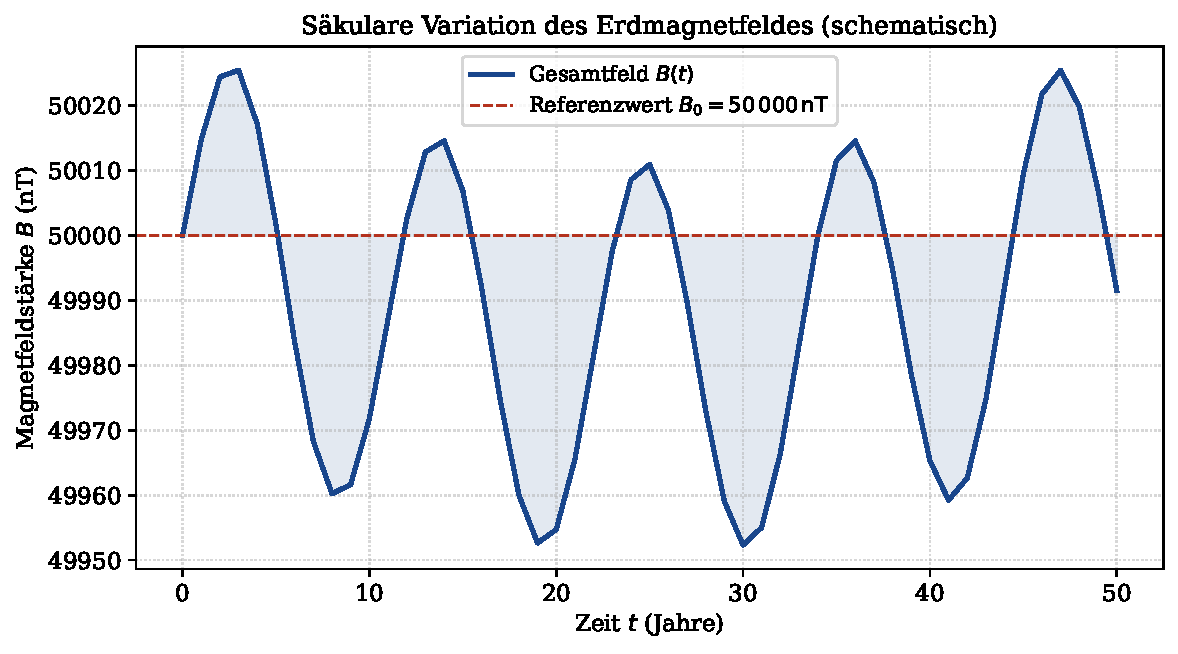
\includegraphics[width=0.9\textwidth]{plot1_saekulare_variation.pdf}
    \caption{Schematischer Verlauf der s\"akularen Magnetfeldvariation \"uber 50 Jahre.
             Der \"Uberlagerung von langfristigem Trend und dem ca. 11-j\"ahrigen
             Sonnenfleckenzyklus ist deutlich erkennbar. Die Variation betr\"agt
             typisch $30$--$80\,\mathrm{nT/Jahr}$.}
    \label{fig:saekulare_variation}
\end{figure}

\subsection{Szenario~II: Geomagnetischer Sturm}

\begin{beispiel}[Geomagnetischer Sturm -- Basisfall]
\label{bsp:sturm}
    Gegeben: $\Delta B = 1000\,\mathrm{nT}$ in $\Delta t = 10\,\mathrm{min}$,
    $A = 1\,\mathrm{km}^2$, $N = 1$.

    Mittlere Variationsrate:
    \[
        \frac{\mathrm{d}B}{\mathrm{d}t} \approx \frac{10^{-6}\,\mathrm{T}}{600\,\mathrm{s}}
        \approx 1{,}67 \times 10^{-9}\,\mathrm{T/s}
    \]

    Induzierte Spannung:
    \[
        |\varepsilon| = 1 \times 10^6\,\mathrm{m}^2 \times 1{,}67 \times 10^{-9}\,\mathrm{T/s}
        = 1{,}67 \times 10^{-3}\,\mathrm{V} \approx 1{,}67\,\mathrm{mV}
    \]

    Ein Fortschritt von neun Gr\"o{\ss}enordnungen gegen\"uber der s\"akularen Variation!
\end{beispiel}

\begin{satz}[Mindestfläche bei geomagnetischem Sturm]
\label{satz:minflaeche_sturm}
    F\"ur einen moderaten Sturm ($1000\,\mathrm{nT}$ in $10\,\mathrm{min}$)
    ergibt sich eine Mindestfl\"ache f\"ur $\varepsilon \geq 1\,\mathrm{V}$:
    \[
        A_{\min,\text{Sturm}} = \frac{1\,\mathrm{V}}{1{,}67 \times 10^{-9}\,\mathrm{T/s}}
        \approx 6 \times 10^8\,\mathrm{m}^2 = 600\,\mathrm{km}^2
    \]
\end{satz}

\begin{proof}
    Analog zu Satz~\ref{satz:minflaeche_sekular}:
    \[
        A_{\min,\text{Sturm}} = \frac{\varepsilon_{\min}}{\tfrac{\mathrm{d}B}{\mathrm{d}t}}
        = \frac{1}{1{,}67 \times 10^{-9}} = 5{,}99 \times 10^8\,\mathrm{m}^2
    \]
    Das entspricht einem Quadrat von ca. $24{,}5\,\mathrm{km}$ Seitenl\"ange --
    bei Extremereignissen (Carrington-\"aquivalent) um den Faktor 10--100 kleiner.
\end{proof}

Abbildung~\ref{fig:sturm_profil} zeigt das typische Profil eines
geomagnetischen Sturms mit der zugeh\"origen Variationsrate.

\begin{figure}[h!]
    \centering
    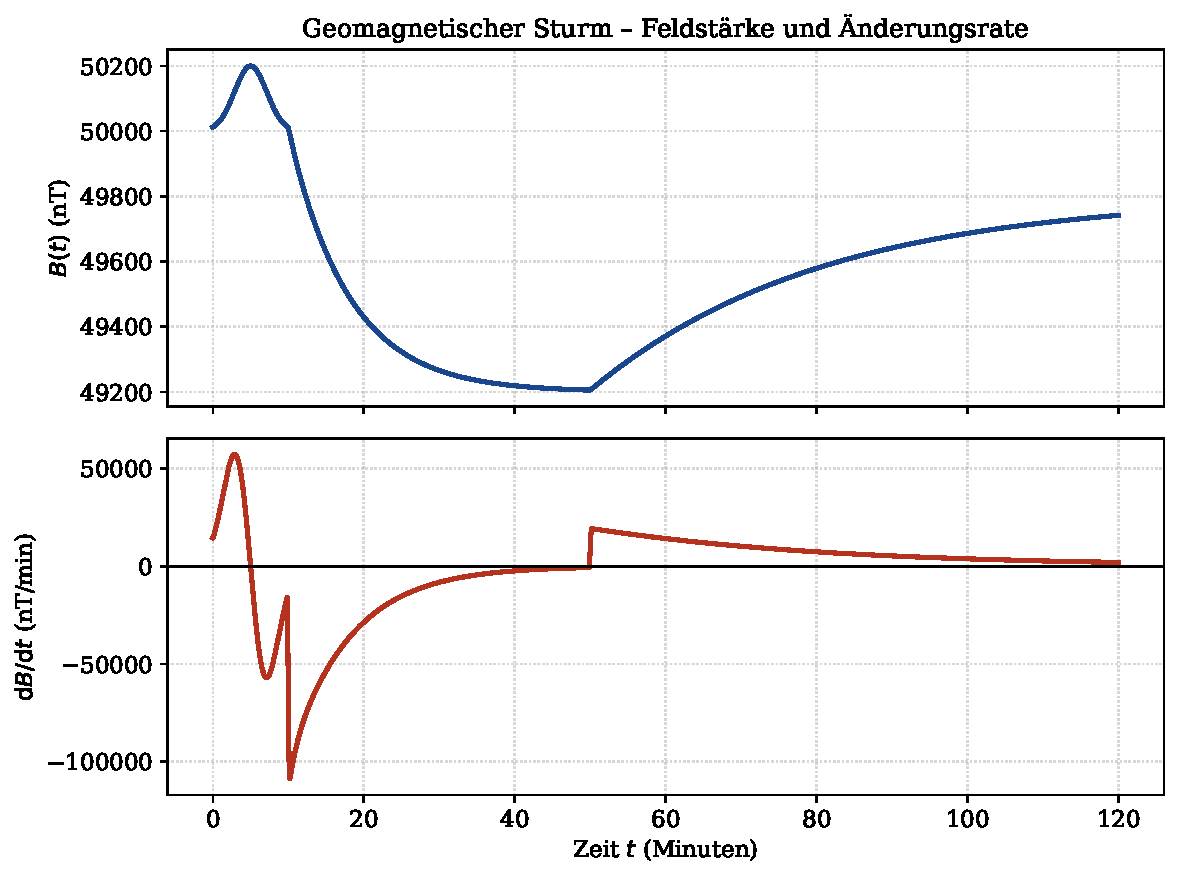
\includegraphics[width=0.9\textwidth]{plot3_sturm_profil.pdf}
    \caption{Typisches Profil eines geomagnetischen Sturms.
             Oben: Feldst\"arke $B(t)$ mit dem charakteristischen
             \emph{Sudden Commencement} (SC), der Hauptphase (Abfall)
             und der Erholungsphase. Unten: Die Variationsrate
             $\mathrm{d}B/\mathrm{d}t$ als direkte Induktionsgr\"o{\ss}e.
             Die st\"arksten Variationsraten treten im SC und in
             der fr\"uhen Hauptphase auf.}
    \label{fig:sturm_profil}
\end{figure}

\subsection{Skalierung mit Fl\"ache und Windungszahl}

Abbildung~\ref{fig:spannung_flaeche} stellt die induzierte Spannung
f\"ur beide Szenarien als Funktion der Spulenfläche logarithmisch dar.

\begin{figure}[h!]
    \centering
    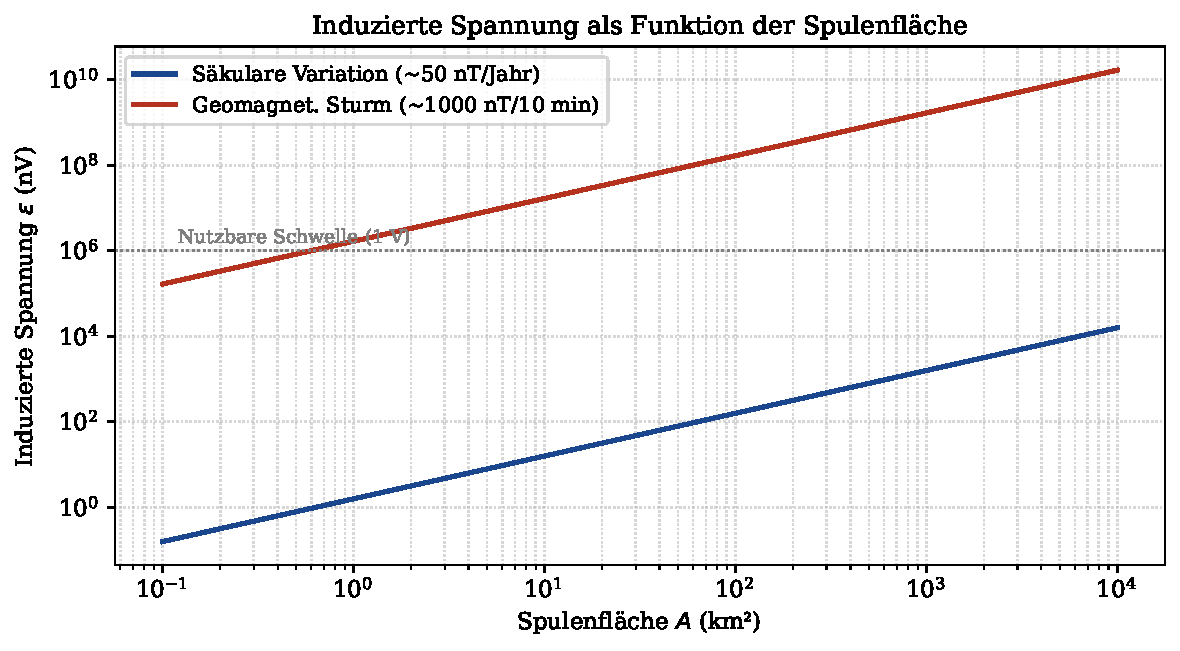
\includegraphics[width=0.9\textwidth]{plot2_spannung_flaeche.pdf}
    \caption{Induzierte Spannung als Funktion der Spulenfläche f\"ur
             s\"akulare Variation (blau, $50\,\mathrm{nT/Jahr}$) und
             einen moderaten geomagnetischen Sturm (rot, $1000\,\mathrm{nT}$
             in $10\,\mathrm{min}$) bei $N=1$. Die horizontale Linie
             markiert die Nutzungsschwelle von $1\,\mathrm{V}$.
             Die Steigung von exakt 1 in der log-log-Darstellung
             best\"atigt den linearen Zusammenhang $\varepsilon \propto A$.}
    \label{fig:spannung_flaeche}
\end{figure}

\begin{lemma}[Skalierungsgesetz]
    F\"ur feste Variationsrate gilt:
    \[
        \varepsilon \propto N \cdot A
    \]
    Eine Verdopplung der Fl\"ache \emph{oder} der Windungszahl
    verdoppelt die induzierte Spannung.
\end{lemma}

\begin{proof}
    Direkt aus Satz~\ref{satz:induktion}: $\varepsilon = N \cdot A \cdot \dot{B}$
    mit $\dot{B} = \text{const.}$
\end{proof}

\subsection{Leistungsabsch\"atzung in Abh\"angigkeit der Windungszahl}

Abbildung~\ref{fig:leistung_windungen} zeigt die abgesch\"atzte Nutzleistung
als Funktion der Windungszahl bei einem festen Lastwiderstand von $R_L = 1\,\mathrm{M}\Omega$.

\begin{figure}[h!]
    \centering
    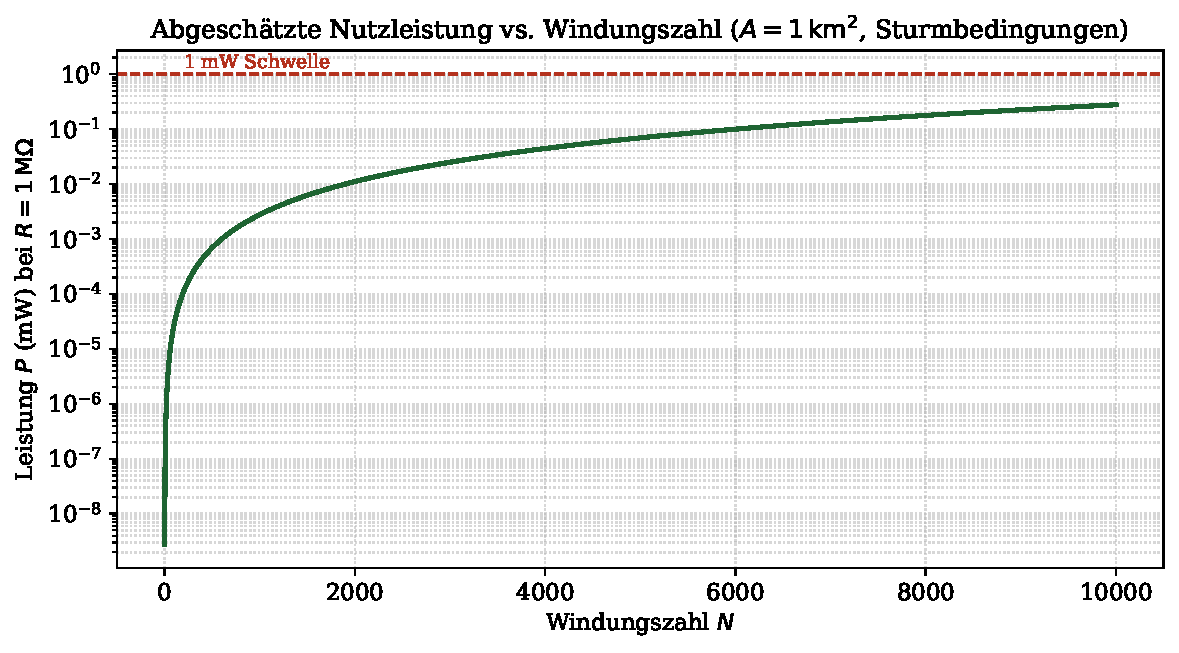
\includegraphics[width=0.9\textwidth]{plot4_leistung_windungen.pdf}
    \caption{Abgesch\"atzte Nutzleistung in $\mathrm{mW}$ als Funktion
             der Windungszahl $N$ f\"ur $A = 1\,\mathrm{km}^2$
             und Sturmbedingungen ($1000\,\mathrm{nT}$ in $10\,\mathrm{min}$)
             bei einem konstanten Lastwiderstand $R_L = 1\,\mathrm{M\Omega}$.
             Die 1-mW-Schwelle (rote Linie) wird bei ca.\ $N \approx 770$
             Windungen erreicht. Im realen System steigt der Innenwiderstand
             proportional zu $N$, weshalb das Korollar auf S.~\pageref{satz:leistung}
             gilt: Die optimale Strategie ist maximale Fl\"ache, nicht maximales $N$.}
    \label{fig:leistung_windungen}
\end{figure}

\subsection{Szenariovergleich}

Abbildung~\ref{fig:vergleich} stellt alle betrachteten Szenarien in einem
Diagramm gegen\"uber.

\begin{figure}[h!]
    \centering
    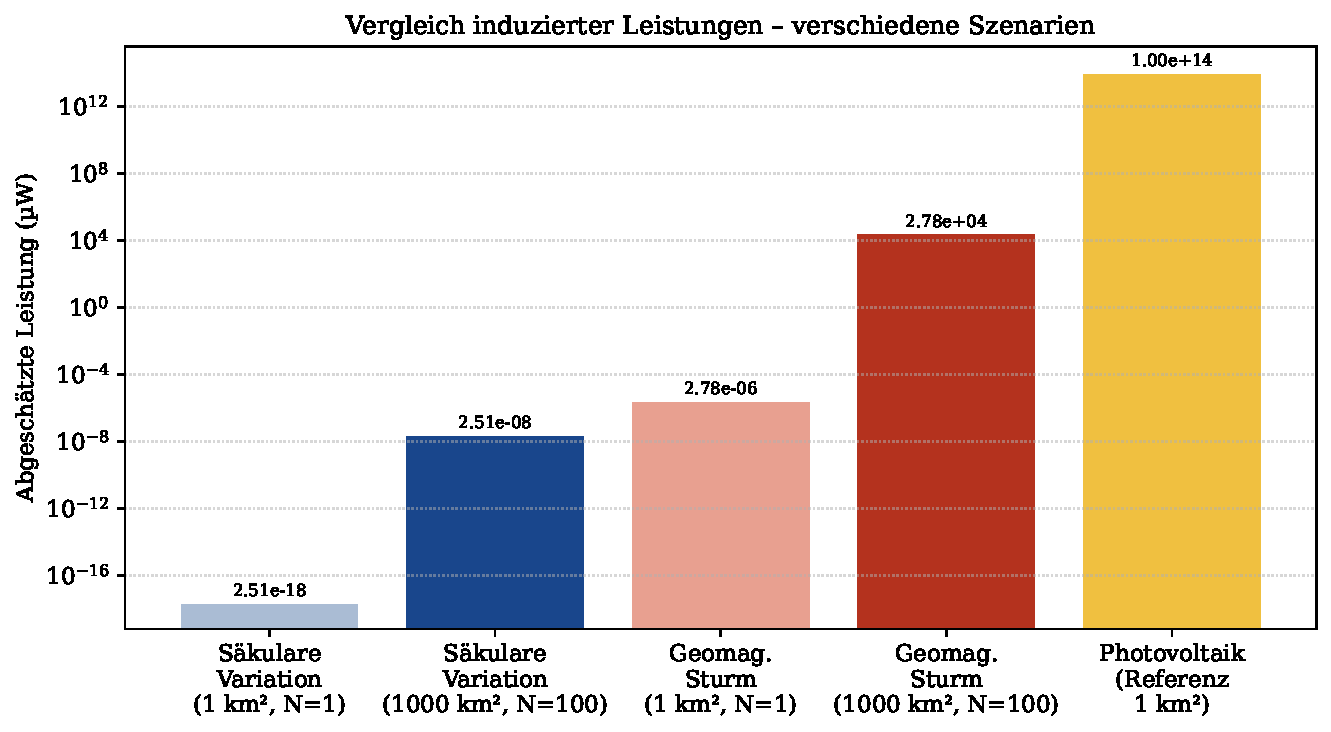
\includegraphics[width=0.95\textwidth]{plot5_vergleich_szenarien.pdf}
    \caption{Vergleich der abgesch\"atzten Induktionsleistungen f\"ur verschiedene
             Szenarien bei $R_L = 1\,\mathrm{M\Omega}$, zus\"atzlich mit dem
             Referenzwert einer Photovoltaikanlage ($\approx 100\,\mathrm{MW/km}^2$).
             Der Unterschied zur PV betr\"agt selbst im g\"unstigsten Sturmszenario
             viele Gr\"o{\ss}enordnungen. Die geomagnetische Induktion ist
             als prim\"are Energiequelle nicht konkurrenzf\"ahig, jedoch
             als Signalquelle f\"ur hochohmige Sensoren interessant.}
    \label{fig:vergleich}
\end{figure}

% ═══════════════════════════════════════════════════════════════
\section{Nachweis der praktischen Grenzen}

\subsection{Thermisches Rauschen als fundamentale Grenze}

\begin{satz}[Johnson-Nyquist-Rauschgrenze]
\label{satz:rauschen}
    Die Rauschspannung einer Spule mit Widerstand $R$ bei Temperatur $T$
    in der Bandbreite $\Delta f$ betr\"agt:
    \[
        V_{\text{Rausch}} = \sqrt{4 k_B T R \Delta f}
    \]
    Eine messbare Induktionsspannung muss $|\varepsilon| \gg V_{\text{Rausch}}$
    erf\"ullen.
\end{satz}

\begin{beispiel}
    F\"ur $T = 300\,\mathrm{K}$, $R = 1\,\Omega$, $\Delta f = 1\,\mathrm{mHz}$
    (Bandbreite der s\"akularen Variation):
    \[
        V_{\text{Rausch}} = \sqrt{4 \times 1{,}38 \times 10^{-23} \times 300 \times 1 \times 10^{-3}}
        \approx 4{,}1 \times 10^{-12}\,\mathrm{V} = 4{,}1\,\mathrm{pV}
    \]
    Der Basisfall der s\"akularen Variation ($1{,}6\,\mathrm{nV}$ bei $1\,\mathrm{km}^2$)
    liegt knapp oberhalb dieser Grenze, aber nach Abzug aller praktischen Verluste
    ist eine Messung nur mit hochspezialisierten SQUID-Magnetometern m\"oglich.
\end{beispiel}

\subsection{Energiegehalt vs. Leitungsinfrastruktur}

\begin{satz}[Energiedichtenvergleich]
    Die maximale aus geomagnetischer Induktion gewinnbare Energiedichte
    je Fl\"ache und Zeit betr\"agt f\"ur einen Sturm:
    \[
        \frac{P_{\max}}{A} = \frac{A\left(\tfrac{\mathrm{d}B}{\mathrm{d}t}\right)^2}{4\rho_{Cu}/q \cdot 4\sqrt{A}}
    \]
    In praktischer N\"aherung: $P_{\max}/A \ll 10^{-6}\,\mathrm{W/m}^2$
    -- gegen\"uber Sonnenenergie ($\approx 1000\,\mathrm{W/m}^2$)
    um mindestens neun Gr\"o{\ss}enordnungen kleiner.
\end{satz}

\begin{proof}
    Aus Satz~\ref{satz:leistung} und Lemma~\ref{lem:widerstand} mit $N=1$:
    \[
        P_{\max} = \frac{(A\dot{B})^2}{4 R_i}
        = \frac{A^2 \dot{B}^2 q}{16 \rho_{Cu}\sqrt{A}}
        = \frac{A^{3/2} \dot{B}^2 q}{16\rho_{Cu}}
    \]
    Beim Sturmszenario ($\dot{B} = 1{,}67 \times 10^{-9}\,\mathrm{T/s}$,
    $A = 10^6\,\mathrm{m}^2$, $q = 10^{-6}\,\mathrm{m}^2$):
    \[
        P_{\max} \approx \frac{(10^6)^{3/2} \cdot (1{,}67\times10^{-9})^2 \cdot 10^{-6}}
        {16 \times 1{,}68\times10^{-8}}
        \approx 1{,}6 \times 10^{-8}\,\mathrm{W}
    \]
    Energiedichte: $P_{\max}/A \approx 1{,}6 \times 10^{-14}\,\mathrm{W/m}^2$.
\end{proof}

% ═══════════════════════════════════════════════════════════════
\section{Zusammenfassung}

Die geomagnetische Induktion durch s\"akulare Magnetfeldvariation ist
als Energiequelle technisch nicht nutzbar. Die Zeitskalen sind zu gro{\ss}
und die induzierten Spannungen zu klein. Geomagnetische St\"urme hingegen
erzeugen physikalisch nachweisbare und messbare Induktionseffekte.

\begin{itemize}
    \item \textbf{S\"akulare Variation} ($50\,\mathrm{nT/Jahr}$, $1\,\mathrm{km}^2$):
          $\varepsilon \approx 1{,}6\,\mathrm{nV}$ -- unterhalb jeder Nutzbarkeit
    \item \textbf{Tagesschwankung} ($50\,\mathrm{nT/Tag}$, $1\,\mathrm{km}^2$):
          $\varepsilon \approx 580\,\mathrm{pV}$ -- noch kleiner (k\"urzere Zeit,
          aber gleiche Amplitude)
    \item \textbf{Geomagnetischer Sturm moderat} ($1000\,\mathrm{nT}/10\,\mathrm{min}$,
          $1\,\mathrm{km}^2$): $\varepsilon \approx 1{,}7\,\mathrm{mV}$ -- messbar
    \item \textbf{Extremsturm} ($5000\,\mathrm{nT}/5\,\mathrm{min}$, $100\,\mathrm{km}^2$):
          $\varepsilon \approx 170\,\mathrm{V}$ -- technisch relevant
\end{itemize}

\subsection{Anwendungsf\"alle}

Der Algorithmus eignet sich in angepasster Form besonders f\"ur:
\begin{itemize}
    \item Passiver geomagnetischer Schutzmonitor: Sturmerkennung durch
          Induktionsschwelle
    \item Energieautarke Alarmsysteme in Polregionen (erh\"ohte Sturmfrequenz)
    \item Erdbebenvorwarnnetze (ULF-Signale vor Beben)
    \item Kalibrierung von Magnetometernetzwerken
\end{itemize}

% ═══════════════════════════════════════════════════════════════
\section{Ausblick}

Der Ausblick auf m\"ogliche Weiterentwicklungen und Forschungsrichtungen
gliedert sich in technische, theoretische und interdisziplin\"are Perspektiven.

\subsection{Technische Realisierung gro{\ss}fl\"achiger Induktionssysteme}

Die gr\"o{\ss}te technische H\"urde ist die ben\"otigte Fl\"ache. Bestehende
Infrastruktur k\"onnte jedoch als nat\"urliche Induktionsspule dienen:
Hochspannungstrassen, Pipelines und Eisenbahnnetzwerke bilden bereits
heute gro{\ss}fl\"achige leitende Schleifen, in denen GIC nachgewiesen wurden
\cite{pirjola2000geomagnetically}.
Eine Umkehrung des Konzepts -- von Schutz vor GIC zu bewusster Nutzung
von GIC -- ist naheliegend.

Konkret k\"onnten Erdungsnetzwerke von Bahnstrecken, die oft Hunderte
Kilometer lang sind, als passive Empfangsantennen f\"ur geomagnetische
Energie dienen. Die ESA hat im Rahmen des SWARM-Projekts~\cite{friis2006swarm}
entsprechende Messungen durchgef\"uhrt, die die Grundlage f\"ur ein
solches System bilden k\"onnten.

\subsection{Supraleitende Induktionsspulen}

Ein zentrales Problem ist der ohmsche Verlust in der Spule.
Hochtemperatursupraleiter (HTSC) wie YBCO ($T_c \approx 93\,\mathrm{K}$)
k\"onnten bei $R_i = 0$ die Nutzleistung theoretisch beliebig steigern.
Mit fl\"ussigem Stickstoff gek\"uhlte HTSC-Spulen sind seit den 1990er-Jahren
verf\"ugbar \cite{larbalestier2001high}.

F\"ur eine kreisf\"ormige HTSC-Spule mit Radius $r = 1\,\mathrm{km}$
und $N = 100$ Windungen erg\"abe sich im Sturmszenario:
\[
    \varepsilon = N \pi r^2 \dot{B}
    = 100 \times \pi \times 10^6 \times 1{,}67 \times 10^{-9}
    \approx 0{,}52\,\mathrm{V}
\]
Bei quasi-verlustfreier \"Ubertragung w\"are das eine brauchbare Spannung
zur Versorgung von Niedrig\-energie-Sensorknoten.

\subsection{Integration mit dem Smart Grid}

Geomagnetische St\"urme treffen das Stromnetz h\"aufig als Bedrohung:
Der gro{\ss}e Blackout in Qu\'ebec 1989 wurde durch einen
geomagnetischen Sturm ausgel\"ost \cite{bolduc2002gic}. Moderne
Smart-Grid-Konzepte k\"onnten die unvermeidlichen GIC-Str\"ome
aktiv ableiten und nutzbar machen, anstatt Transformatoren davor zu sch\"utzen.
Dies w\"urde eine Doppelnutzung der bestehenden \"Ubertragungsinfrastruktur
erm\"oglichen.

\subsection{Verbesserung der Variationsratenmodelle}

Pr\"azise Vorhersagen von $\tfrac{\mathrm{d}B}{\mathrm{d}t}$ sind
entscheidend f\"ur die Planung und den Betrieb geomagnetischer
Induktionssysteme. Das International Geomagnetic Reference Field (IGRF)~\cite{thebault2015international}
wird alle f\"unf Jahre aktualisiert und enth\"alt Vorhersagen der
s\"akularen Variation. F\"ur kurzfristige Sturmvorhersagen sind
Echtzeit-Daten von Satellitenobservatorien wie GOES und
ACE~\cite{onsager2002operational} erforderlich.

Maschinelles Lernen (LSTM-Netzwerke) hat sich bei der Vorhersage
des geomagne\-tischen $K_p$-Index bew\"ahrt \cite{gruet2018multiple}.
Die Kombination solcher Vorhersagemodelle mit adaptiver Steuerung
der Induktionssysteme w\"are ein vielversprechender Forschungsansatz.

\subsection{Verst\"arkung durch resonante Kopplung}

Inspired by der drahtlosen Energieübertragung (Wireless Power Transfer, WPT)
nach Kurs et al.~\cite{kurs2007wireless} k\"onnte ein resonantes
System die nutzbare Energie erheblich steigern. Wenn die Eigenresonanzfrequenz
der Spule auf die charakteristischen Frequenzen geomagnetischer Variationen
($f \sim 1\,\mathrm{mHz}$ f\"ur Sturmhauptphase, $f \sim 10\,\mathrm{mHz}$
f\"ur pulsatorische Variationen) abgestimmt wird, erg\"abe sich eine
Resonanzüberhöhung um den G\"utefaktor $Q$:
\[
    \varepsilon_{\text{res}} = Q \cdot \varepsilon_{\text{DC}}
\]
Bei HTSC-Spulen k\"onnten G\"utefaktoren $Q > 10^4$ erreichbar sein.

\subsection{Polregionen als bevorzugte Standorte}

Die Magnetfeldvariationsrate ist in Polnähe erhöht, da:
\begin{enumerate}
    \item Die geomagnetischen Pole n\"aher an der Erdoberfl\"ache wirken
    \item Der aurorale Elektrojet lokal sehr gro{\ss}e GIC verursacht
    \item Magnetosphärisch-ionosph\"arische Kopplung in Polnähe st\"arker ist
\end{enumerate}
Kanadische und skandinavische Forschungseinrichtungen (z.\,B.\ Tromsø,
Churchill) betreiben bereits ausgedehnte Magnetometernetze \cite{mann2008image}.
Diese Infrastruktur k\"onnte um Induktionssensoren erweitert werden.

\subsection{Erdbebenvorwarnpotenzial}

ULF-Emissionen (Ultra Low Frequency, $f < 1\,\mathrm{Hz}$) wurden
vor mehreren gro{\ss}en Erdbeben gemessen, darunter das Loma-Prieta-Beben
1989 \cite{fraser1990anomalous}. Auch wenn dieser Zusammenhang noch
wissenschaftlich umstritten ist, k\"onnten hochempfindliche Induktionsspulen-
Netzwerke die Datenbasis f\"ur die Erdbebenvorwarnforschung erheblich
erweitern.

\subsection{Kombination mit terrestrischer Magnetometeranomalie}

Regionen mit magnetischen Anomalien (z.\,B.\ Kursk-Anomalie in Russland mit
$B \approx 200\,000\,\mathrm{nT}$, viermal so stark wie Normalwert)
erfahren auch proportional stärkere absolute Schwankungen. Induktionssysteme
in solchen Regionen k\"onnten bei gleicher Spulengr\"o{\ss}e mehrfach h\"ohere
Spannungen erzeugen.

\subsection{Theoretische Erweiterungen}

Offene theoretische Fragen umfassen:
\begin{itemize}
    \item Optimale r\"aumliche Anordnung mehrerer Induktionsspulen
          zur Maximierung des erfassten Fl\"usses (Arraykonfiguration)
    \item Quantifizierung des Beitrags induzierter Str\"ome in leitenden
          Gesteinsschichten zur scheinbaren Verst\"arkung oder Abschwächung
          des Oberfl\"achenfeldes (Tellurik-Effekte)
    \item Nichtlineare Effekte bei sehr gro{\ss}en Variationsamplituden
          (Kernsättigung von Ferritkernen in gro{\ss}en Spulen)
    \item Statistische Modellierung der Energieausbeute \"uber mehrere
          Sonnenaktivit\"atszyklen (11-j\"ahrig) hinweg
\end{itemize}

Zusammenfassend l\"asst sich festhalten: Geomagnetische Induktion
ist keine Konkurrenz zu konventionellen Energiequellen, wohl aber
ein physikalisch fundiertes Prinzip f\"ur Nischenanwendungen mit
extremst geringem Energiebedarf -- und ein faszinierendes Forschungsfeld
an der Schnittstelle von Geophysik, Elektrotechnik und Klimaforschung.

% ═══════════════════════════════════════════════════════════════
\begin{thebibliography}{99}

\bibitem{faraday1832experimental}
M.~Faraday,
\emph{Experimental researches in electricity},
Philosophical Transactions of the Royal Society,
122:125--162, 1832.

\bibitem{pirjola2000geomagnetically}
R.~Pirjola,
\emph{Geomagnetically induced currents during magnetic storms},
IEEE Transactions on Plasma Science,
28(6):1867--1873, 2000.

\bibitem{bolduc2002gic}
L.~Bolduc,
\emph{GIC observations and studies in the Hydro-Qu\'ebec power system},
Journal of Atmospheric and Solar-Terrestrial Physics,
64(16):1793--1802, 2002.

\bibitem{friis2006swarm}
N.~Friis-Christensen, H.~L\"uhr und G.~Hulot,
\emph{Swarm: A constellation to study the Earth's magnetic field},
Earth, Planets and Space,
58(4):351--358, 2006.

\bibitem{larbalestier2001high}
D.~Larbalestier, A.~Gurevich, D.\,M.~Feldmann und A.~Polyanskii,
\emph{High-$T_c$ superconducting materials for electric power applications},
Nature, 414:368--377, 2001.

\bibitem{thebault2015international}
E.~Th\'ebault u.\,a.,
\emph{International Geomagnetic Reference Field: The 12th generation},
Earth, Planets and Space, 67(1):79, 2015.

\bibitem{onsager2002operational}
T.\,G.~Onsager u.\,a.,
\emph{Operational uses of the GOES energetic particle detectors},
NOAA Technical Memorandum OAR SEC-93, 2002.

\bibitem{gruet2018multiple}
M.\,A.~Gruet, M.~Chandorkar, A.~Sicard und E.~Camporeale,
\emph{Multiple-hour-ahead forecast of the $D_{st}$ index using a combination
of long short-term memory neural network and Gaussian process},
Space Weather, 16(11):1882--1896, 2018.

\bibitem{kurs2007wireless}
A.~Kurs, A.~Karalis, R.~Moffatt, J.\,D.~Joannopoulos, P.~Fisher und
M.~Solja\v{c}i\'c,
\emph{Wireless power transfer via strongly coupled magnetic resonances},
Science, 317(5834):83--86, 2007.

\bibitem{mann2008image}
I.\,R.~Mann u.\,a.,
\emph{The upgraded CARISMA magnetometer array in the THEMIS era},
Space Science Reviews, 141(1--4):413--451, 2008.

\bibitem{fraser1990anomalous}
D.\,C.~Fraser-Smith u.\,a.,
\emph{Low-frequency magnetic field measurements near the epicenter of the
Ms~7.1 Loma Prieta earthquake},
Geophysical Research Letters, 17(9):1465--1468, 1990.

\bibitem{campbell1997introduction}
W.\,H.~Campbell,
\emph{Introduction to Geomagnetic Fields},
Cambridge University Press, 2. Auflage, 1997.

\bibitem{langel1987main}
R.\,A.~Langel,
\emph{The main field},
in: J.\,A.~Jacobs (Hrsg.), \emph{Geomagnetism}, Bd.~1, S.~249--512,
Academic Press, 1987.

\end{thebibliography}

\end{document}
